% ------------------------------------------------------------------------------
% Apêndice
% ------------------------------------------------------------------------------

	\chapter{Como fazer citações}

		Você pode fazer uma citação de diversas formas. Se você quiser fazer uma citação entre parênteses, você pode fazer assim: \citep{milgram1969note}. Se você quiser mencionar o número da página, você pode fazer assim: \citep[p. 10]{deb2002fast}. Agora, se você quiser fazer uma citação onde o autor é parte da sentença, você pode fazer assim: \cite{maxwell1865viii} afirma que... Se você quiser fazer uma citação com mais de um autor, você pode fazer assim: \citep{van2019fantastic,maxwell1865viii}. \textbf{Pode que ser, às vezes, você tenha que compilar o arquivo mais de uma vez para que as citações apareçam corretamente. Ou até escrever qualquer coisa a mais.}
	
	\chapter{Como escrever equações}

		O LaTeX oferece uma ampla gama de recursos e pacotes para escrever e formatar equações de forma clara e profissional. Além disso, o LaTeX permite referenciar e numerar automaticamente as equações, facilitando a referência cruzada e a organização do conteúdo matemático. Aqui estão alguns exemplos de equações que você pode usar em seu trabalho.

		Um exemplo básico de equação:
		\begin{equation}
			\boldsymbol{\mathcal{F}}(\mathbf{r}, t) = \mathfrak{Re}\{\mathbf{F}(\mathbf{r})e^{j\omega t}\} \label{eq:2:fourier}
		\end{equation}

		Um exemplo sobre como escrever múltiplas equações e o uso de fonte cursiva nas letras:
		\begin{eqnarray}
			\nabla\times\boldsymbol{\mathcal{E}}(\mathbf{r}, t) &=& - \frac{\partial\boldsymbol{ \mathcal{B}}}{\partial t}(\mathbf{r}, t) \label{eq:2:maxwell:time:1} \\
			\nabla\times\boldsymbol{\mathcal{H}}(\mathbf{r}, t) &=& \frac{\partial\boldsymbol{ \mathcal{D}}}{\partial t}(\mathbf{r}, t) + \boldsymbol{\mathcal{J}}(\mathbf{r}, t) \label{eq:2:maxwell:time:2} \\
			\nabla\cdot\boldsymbol{\mathcal{D}}(\mathbf{r}, t) &=& \rho(\mathbf{r}, t) \label{eq:2:maxwell:time:3} \\
			\nabla\cdot\boldsymbol{\mathcal{B}}(\mathbf{r}, t) &=& 0 \label{eq:2:maxwell:time:4}
		\end{eqnarray}

		Um exemplo de desenvolvimento de equação:
		\begin{eqnarray}
			\nabla\times\mathbf{H}(\mathbf{r}) &=&  j\omega\epsilon_0\epsilon_r\mathbf{E}(\mathbf{r}) + \sigma(\mathbf{r})\mathbf{E}(\mathbf{r})+ \mathbf{J}_i(\mathbf{r}) \label{eq:2:complexmedia:1} \\
			 &=&  j\omega\epsilon_0\left(\epsilon_r(\mathbf{r}) -j\frac{\sigma(\mathbf{r})}{\omega\epsilon_0}\right)\mathbf{E}(\mathbf{r}) +  \mathbf{J}_i(\mathbf{r}) \label{eq:2:complexmedia:2} \\
			&=&  j\omega\epsilon(\mathbf{r})\mathbf{E}(\mathbf{r}) +  \mathbf{J}_i(\mathbf{r}) \label{eq:2:complexmedia:3}
		\end{eqnarray}

		Um exemplo de equação quebrada em mais de uma linha:
		\begin{multline}
			\chi(\brho)E_{z_i}(\brho) = J_{z_{eq}}(\brho) + \frac{jk_b^2}{4} \chi(\brho) \int_S dS^\prime J_0(k_b|\brho-\brhop|) J_{z_{eq}}(\brhop) \\ + \frac{jk_b^2}{4} \chi(\brho) \int_S dS^\prime Y_0(k_b|\brho-\brhop|) J_{z_{eq}}(\brhop)  \label{eq:2:2d:greendecomp:csie}
		\end{multline}

		Um exemplo de equação com somatórios e integrais:
		\begin{multline}
			\iint_D E_{z_s}(\theta,\phi) w^{(\theta)}_u(\theta) w^{(\phi)}_v(\phi) d\theta d\phi = \\ -\frac{jk_b^2}{4} \sum\limits_{i=1}^{N_I}\sum\limits_{j=1}^{N_J} \sum\limits_{p=1}^{N_P}\sum\limits_{q=1}^{N_Q}\sum\limits_{r=1}^{N_R} a_{ij} b_{pqr} \iint\limits_{D} \iint\limits_{S} d\theta d\phi dxdy~ \bigg[ G^D_{2D}(\theta,x,y) \\ f^{(x)}_i(x) f^{(y)}_j(y) g^{(x)}_{p}(x) g^{(y)}_{q}(y) g^{(\phi)}_r(\phi)w^{(\theta)}_u(\theta) w^{(\phi)}_v(\phi)  \bigg], \\ u = 1,\cdots, N_U,~ v = 1,\cdots,N_V \label{eq:3:discretization:6}
		\end{multline}

		Um exemplo de definição de matriz:
		\begin{equation}
			\boldsymbol{\bar{\Lambda}} = \begin{bmatrix}
																\Lambda_{11} & \Lambda_{12} & \cdots & \Lambda_{1N_V} \\
															   \Lambda_{21} & \Lambda_{22} & \cdots & \Lambda_{2N_V} \\
															   \vdots & \vdots & \vdots & \vdots \\
															   \Lambda_{u1} & \Lambda_{u2} & \cdots & \Lambda_{uN_V} \\
															   \vdots & \vdots & \vdots & \vdots \\
															   \Lambda_{N_U1} & \Lambda_{N_U2} & \cdots & \Lambda_{N_UN_V}
															  \end{bmatrix} \label{eq:discretization:9}
	   \end{equation}

	   Um exemplo de definição de casos:
	   \begin{equation}
		w_{uv} = \begin{cases}
						  1,& \mathrm{in} ~D_{uv}, \\
						  0,& \mathrm{outside}, ~D_{uv}
					  \end{cases} \label{eq:3:discretization:subdomain}
		\end{equation}

		Um exemplo para organização de três matrizes em uma mesma linha:
		\begin{align}
			\boldsymbol{\bar{\chi}} &=	\begin{bmatrix}
														 \chi_{11} & 0 & \cdots & 0 \\
														 0 & \chi_{12} & \cdots & 0 \\
														 \vdots & \vdots & \ddots & \vdots \\
														  0 & 0 & \cdots & \chi_{N_IN_J}
													 \end{bmatrix}
			&\boldsymbol{\bar{\beta}} &=	\begin{bmatrix}
																\beta_{11} & 0 & \cdots & 0 \\
																0 & \beta_{12} & \cdots & 0 \\
																\vdots & \vdots & \ddots & \vdots \\
																0 & 0 & \cdots & \beta_{N_IN_J}
															\end{bmatrix}
			&\mathbf{\bar{R}} &=	\begin{bmatrix}
													R_{11} & 0 & \cdots & 0 \\
													0 & R_{12} & \cdots & 0 \\
													\vdots & \vdots & \ddots & \vdots \\
													0 & 0 & \cdots & R_{N_IN_J}
												\end{bmatrix} \label{eq:3:discretization:collocation:18}
		\end{align}

		Note que você pode referenciar equações das seguintes formas:

		\begin{itemize}
			\item Quando ela estiver no meio da frase, você pode usar simplesmente o comando \verb|\eqref{}|. Por exemplo: ``...como mostrado em \eqref{eq:2:maxwell:time:1}, ...''
			\item Quando você estiver no início da frase, você pode escrever: ``A Eq. \eqref{eq:2:maxwell:time:1} mostra que...''
		\end{itemize}

		É claro que também é possível digitar equações através do comando \verb|$$ $$|, como por exemplo $$a^2 + b^2 = c^2,$$ mas note que o LaTeX não irá numerar a equação e você não poderá referenciá-la.
		
		Pode ser também que você queira usar o comando \verb|\begin{equation}\end{equation}| e que o texto em seguida não comece em um novo parágrafo. Nesse caso, você pode usar o comando \verb|\noindent| para evitar a quebra de linha. Por exemplo:
		\begin{equation}
			e^{j\pi} + 1 = 0
		\end{equation}
		\noindent a qual é a fórmula de Euler, uma das mais famosas equações da matemática.

	\chapter{Como inserir figuras}

		Um exemplo sobre como inserir figuras simples pode ser visto em \ref{fig:2:scattering}. Você pode referenciar figuras através do comando \verb|\ref{}| ou do comando \verb|\autoref{}|. O primeiro comando apenas referencia o número da figura, enquanto o segundo comando referencia o número da figura e o nome dela. Por exemplo, você pode escrever: ``...como mostrado na \autoref{fig:2:scattering}, ...''.
		\begin{figure}[h]
			\centering
			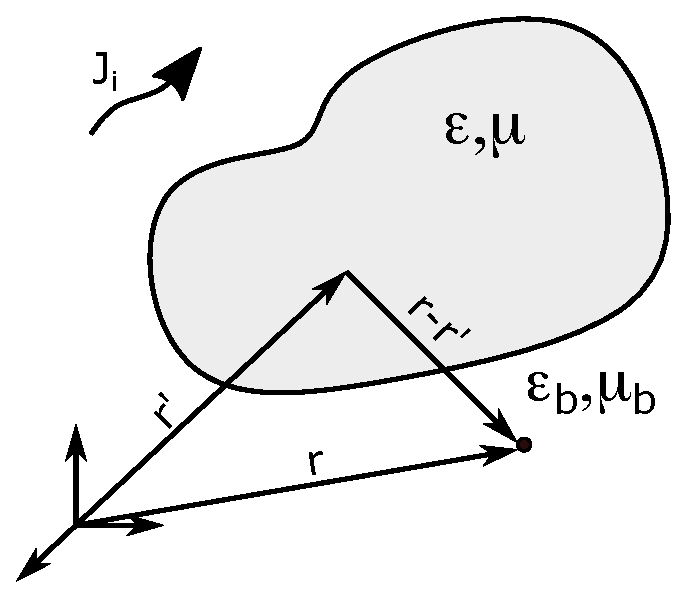
\includegraphics[width=0.5\textwidth]{./figuras/scattering}
			\caption{General scattering problem.}
			\label{fig:2:scattering}
		\end{figure}

		Os comandos de posicionamento de figuras no LaTeX são usados para controlar a posição das figuras em relação ao texto. Existem alguns comandos de posicionamento comumente usados:

		\begin{itemize}
			\item \verb|[h]|: Posiciona a figura ``aqui" (here), ou seja, o mais próximo possível do local onde o comando é inserido no código. No entanto, o LaTeX pode ignorar esse comando se não houver espaço suficiente na página atual para acomodar a figura.
			\item \verb|[t]|: Posiciona a figura no topo (top) da página.
			\item \verb|[b]|: Posiciona a figura na parte inferior (bottom) da página.
			\item \verb|[p]|: Posiciona a figura em uma página separada (page) exclusivamente para figuras.
			\item \verb|[!htb]|: Combina os comandos [h], [t] e [b], permitindo que o LaTeX escolha a melhor posição para a figura entre o topo, a parte inferior e o local onde o comando é inserido.
		\end{itemize}

		É importante observar que esses comandos são sugestões para o LaTeX e não garantem que a figura será posicionada exatamente onde você deseja. O LaTeX tentará encontrar a melhor posição para a figura com base em vários fatores, como espaço disponível na página e ajuste do layout.

		Um exemplo de múltiplas figuras pode ser visto na \autoref{fig:3:lcurve}. Um outro exemplode múltiplas figuras pode ser visto na \autoref{fig:proposed-methodology:surrogate:optimization:objfun}. Um exemplo para inserir duas figuras horizontais é a Figura \ref{fig:results:casestudy:austria:boxplot:zeta_eoe}.

		\begin{figure}[!htb]
			\centering
			\subfloat[]{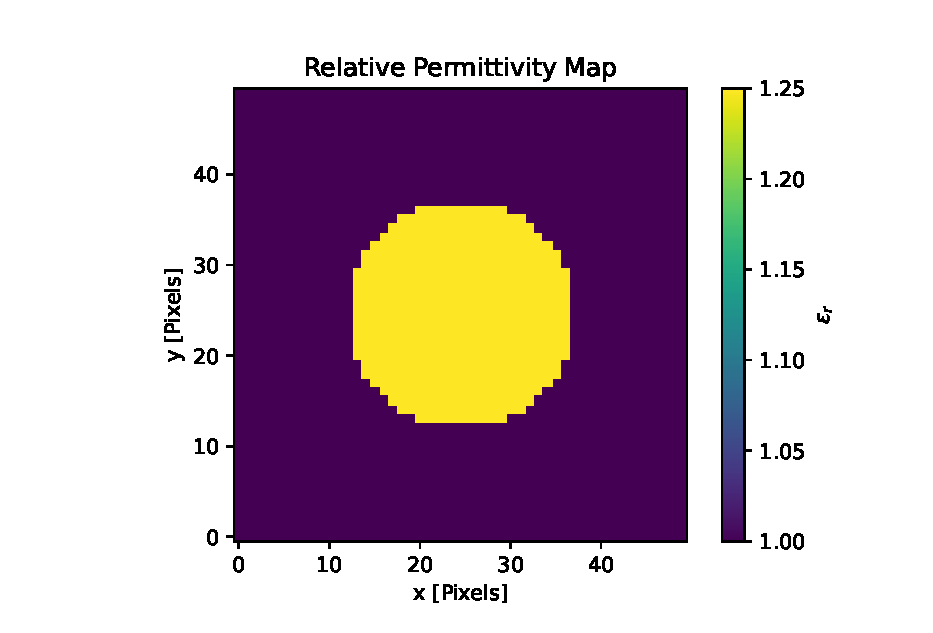
\includegraphics[width=.5\textwidth]{figuras/lcurve_input}}
			\subfloat[]{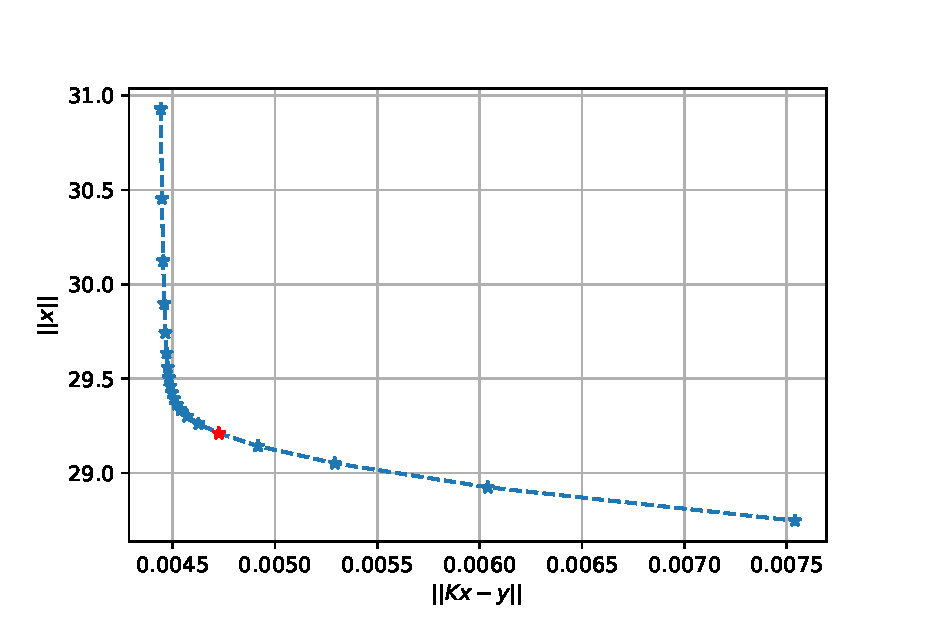
\includegraphics[width=.5\textwidth]{figuras/lcurve}} \\
			\subfloat[]{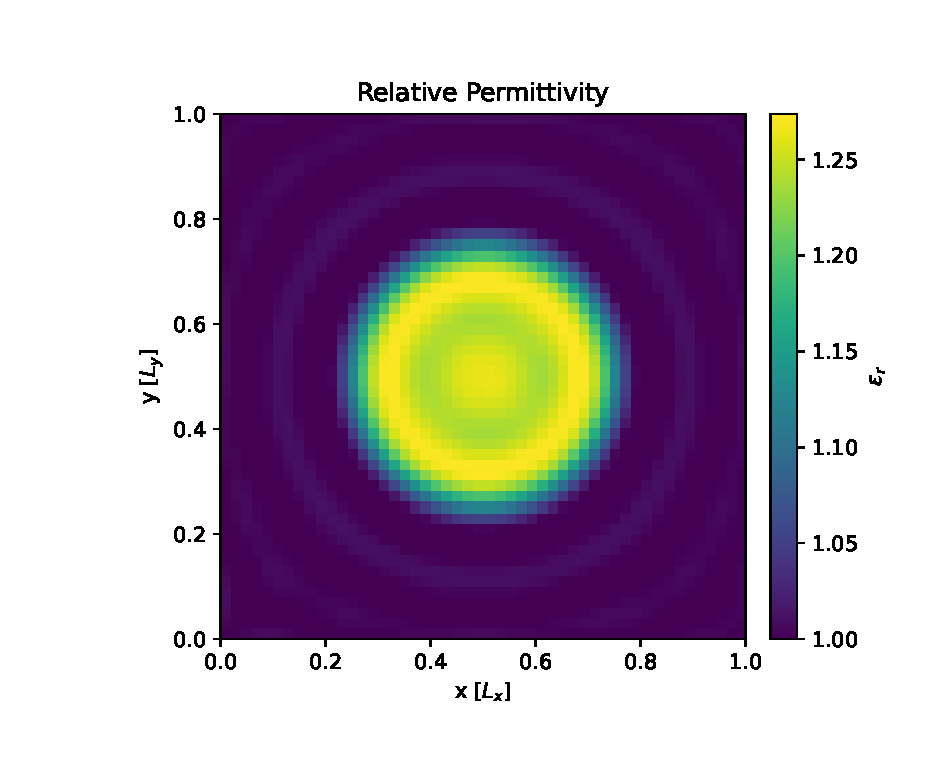
\includegraphics[width=.5\textwidth]{figuras/lcurve_result}}
			\caption[Exemplo de aplicação do Método da Curva-L.]{Example of applying the L-curve Method to a linear problem where it presupposes knowledge of the total field. (a) A simple instance of a contrast dielectric circle $\chi=0.25$ and radius $0.8\lambda_b$. Respecting the degrees of freedom, the scattered field was sampled in 45 positions for 45 incidence angles at a distance of $10\lambda_b$ from the center of the image. (b) L-curve considering 20 values of $\alpha_T$ in a range of $10^{-5}$ a $10^{-2}$. The red dot represents the solution with the shortest normalized distance to the origin. Its $\alpha_T$ value is approximately $2.3357 \times10^{-3}$. (c) Reconstruction of the image using the $\alpha_T$ value from the red dot. No inverse crime was committed since the data were obtained from the analytical solution.}
			\label{fig:3:lcurve}
		\end{figure}

		\begin{figure}[!h]
			\centering
			\subfloat[]{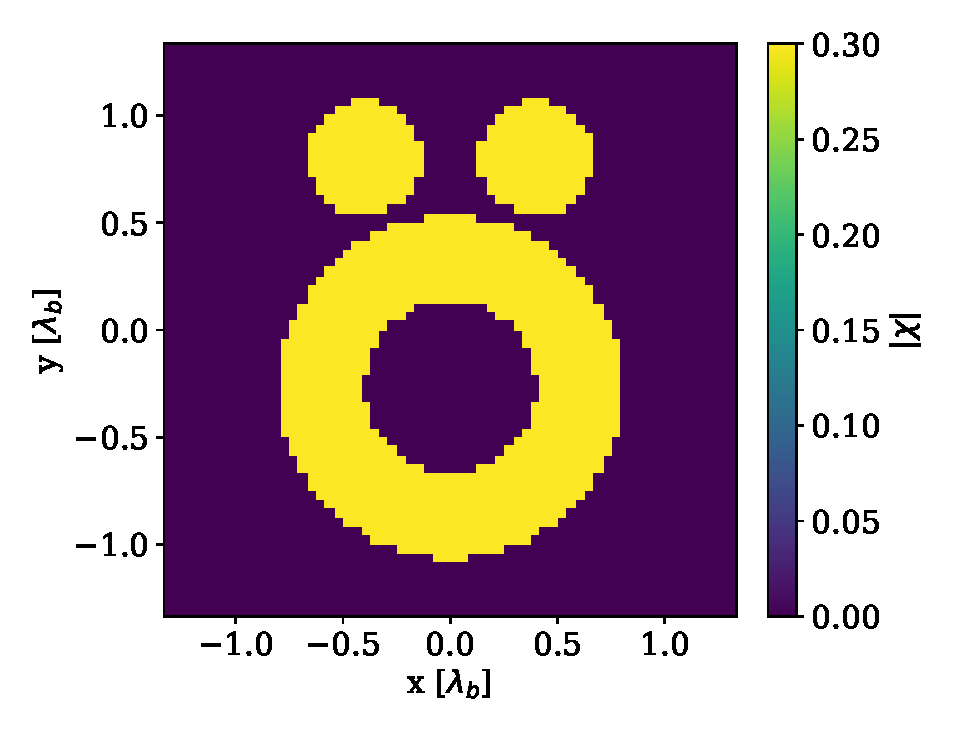
\includegraphics[width=.4\textwidth]{./figuras/objfun_groundtruth}\label{fig:proposed-methodology:surrogate:optimization:objfun:groundtruth}} \hspace{.05\textwidth}
			\subfloat[]{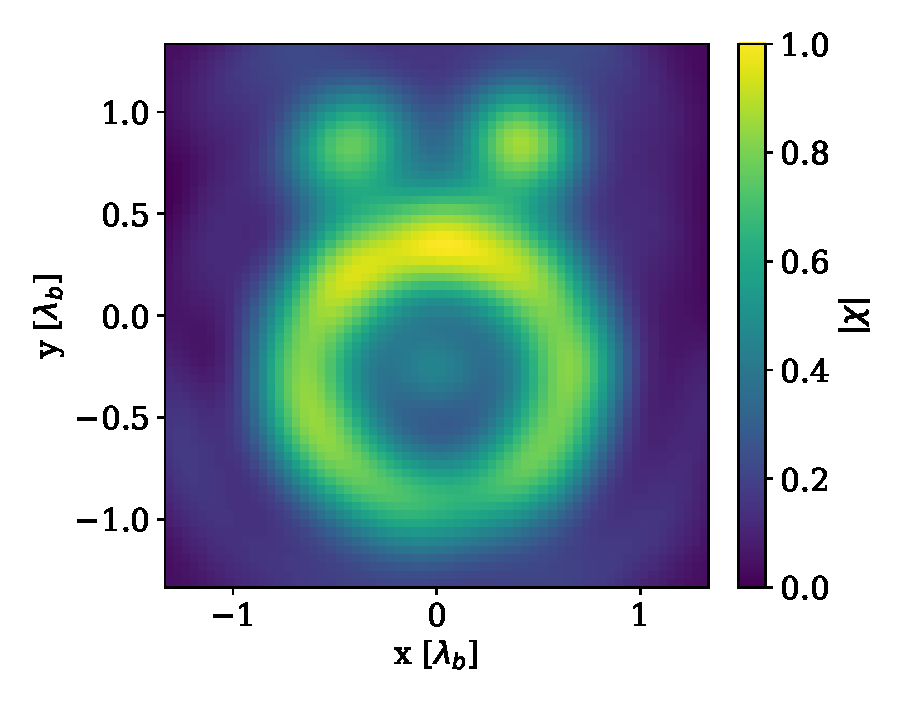
\includegraphics[width=.4\textwidth]{./figuras/objfun_qualitative}\label{fig:proposed-methodology:surrogate:optimization:objfun:qualitative}} \\
			\subfloat[]{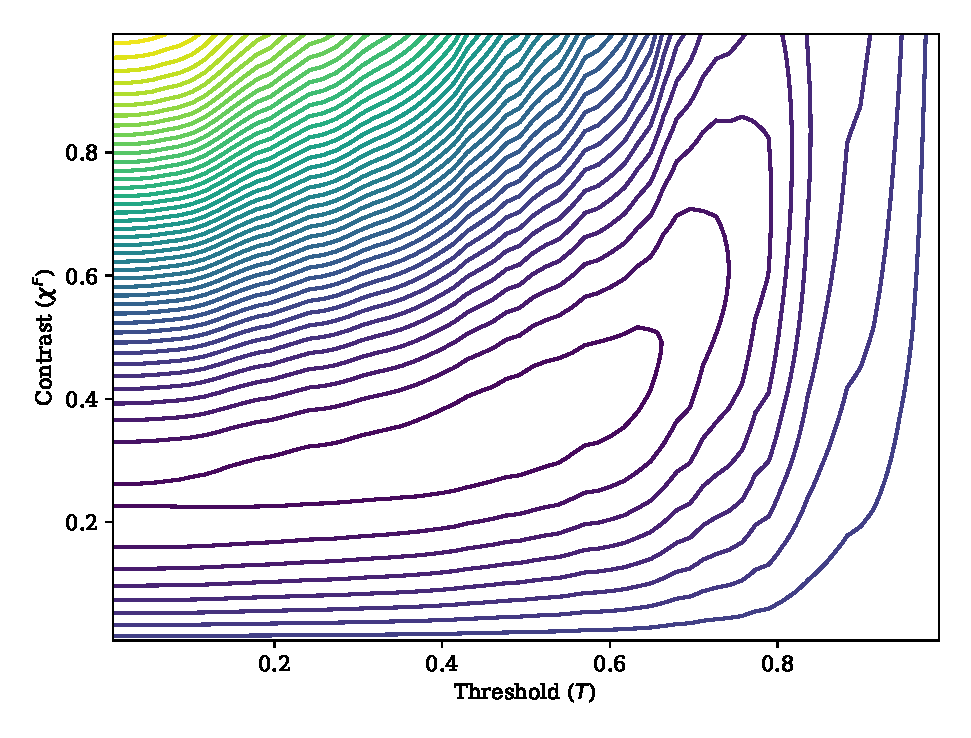
\includegraphics[width=.4\textwidth]{./figuras/objfun_surface}\label{fig:proposed-methodology:surrogate:optimization:objfun:surface}} \hspace{.05\textwidth}
			\subfloat[]{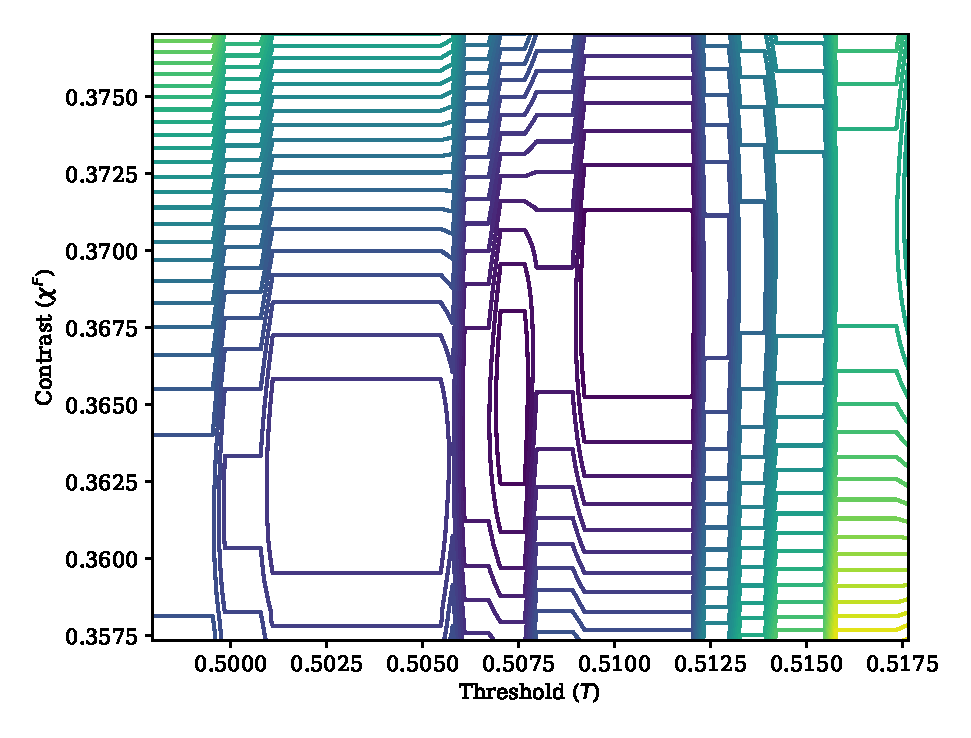
\includegraphics[width=.4\textwidth]{./figuras/objfun_nearoptimum}\label{fig:proposed-methodology:surrogate:optimization:objfun:nearoptimum}}
			\caption[Example of an objective function resulting from the transformation of the inversion problem into a two-dimensional optimization one.]{Example of an objective function resulting from the transformation of the inversion problem into a two-dimensional optimization one: (a) the ground-truth image; (b) the image obtained by OSM; (c) the surface obtained by the transformation of the inversion problem into a two-dimensional optimization one; and (d) a zoom over the region close to the optimum.}
			\label{fig:proposed-methodology:surrogate:optimization:objfun}
		\end{figure}

		
		\begin{figure}
			\centering
			\subfloat[]{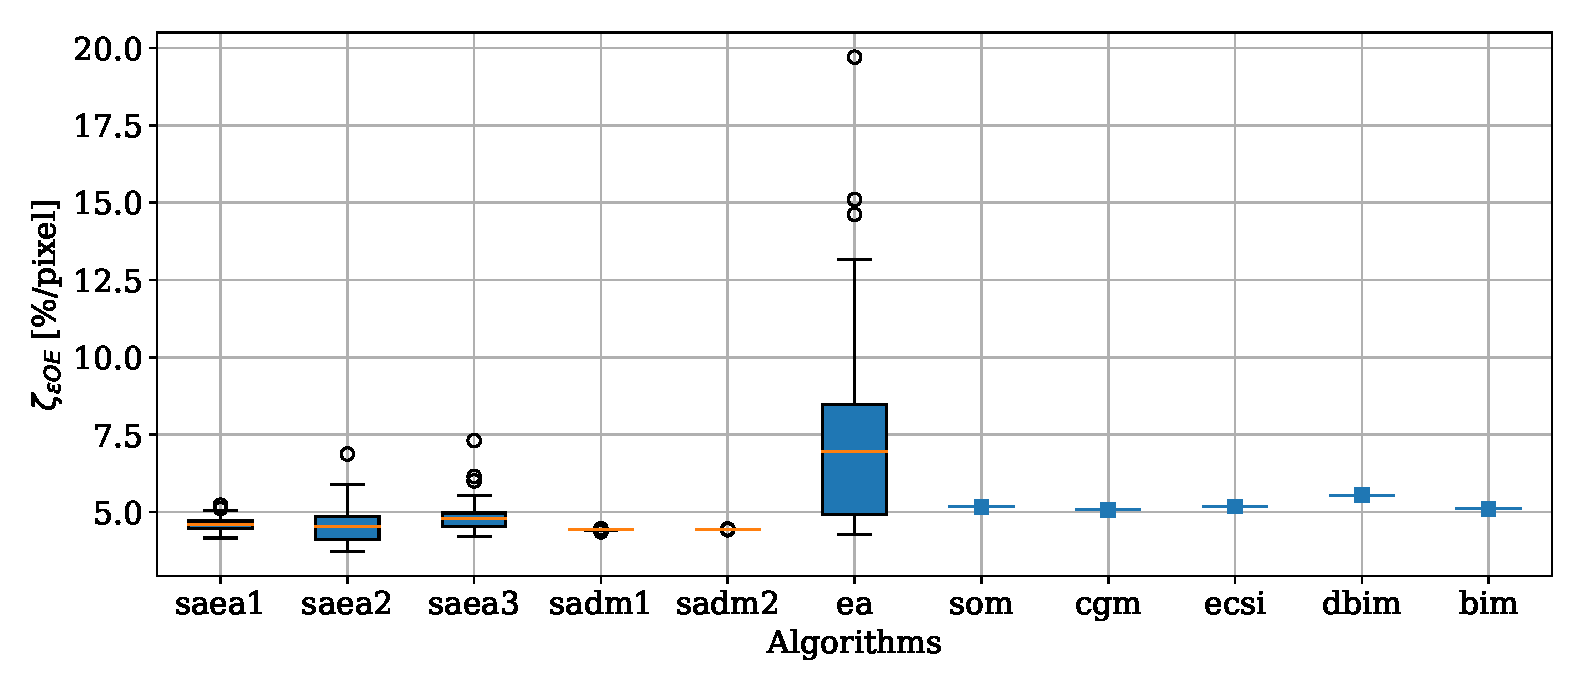
\includegraphics[width=.9\textwidth]{./figuras/boxplot_zeta_eoe_ea}\label{fig:results:casestudy:austria:boxplot:zeta_eoe:withea}} \\
			\subfloat[]{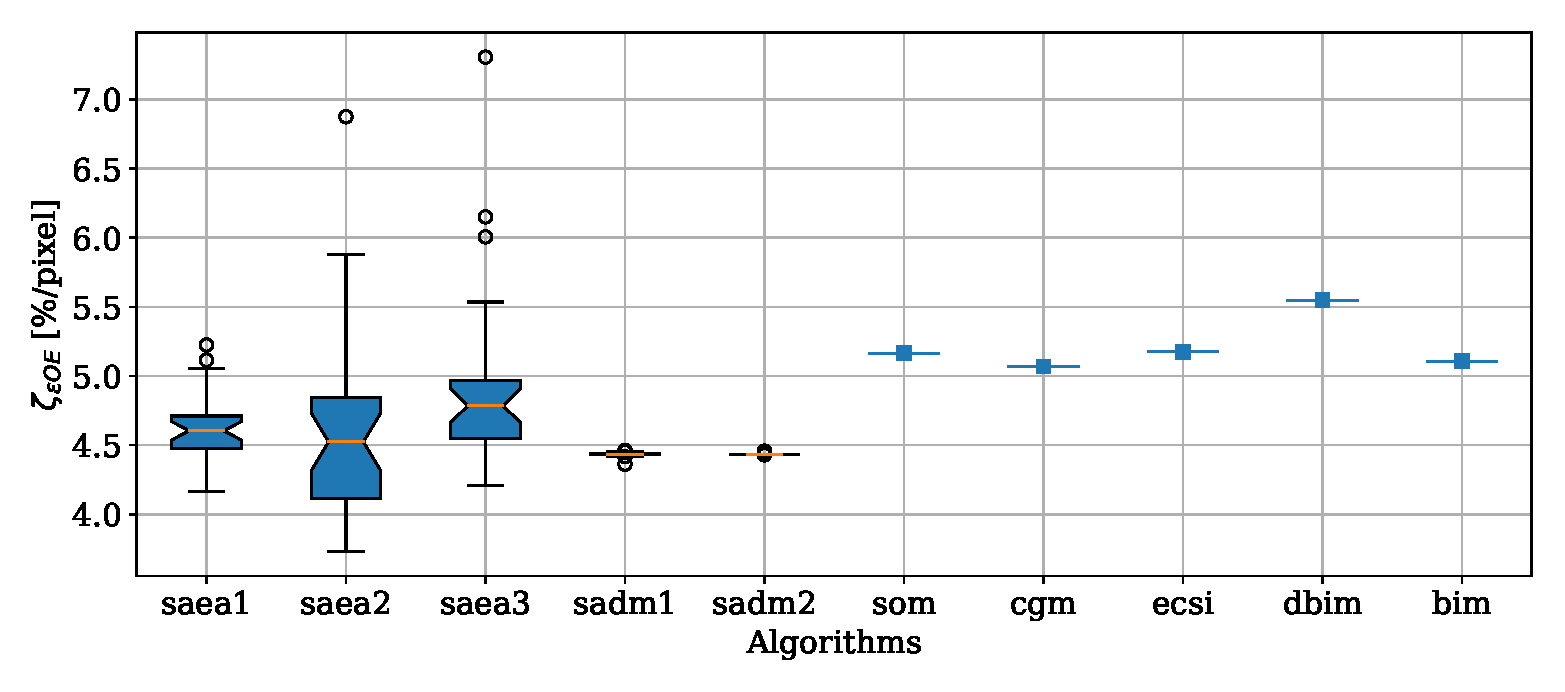
\includegraphics[width=.9\textwidth]{./figuras/boxplot_zeta_eoe}\label{fig:results:casestudy:austria:boxplot:zeta_eoe:noea}}
			\caption[Performance of $\zeta_{\epsilon OE}$ indicator for various algorithms in the Austria profile.]{Performance of $\zeta_{\epsilon OE}$ indicator for various algorithms in the Austria profile. (a) Boxplots show quartiles of 30 executions for stochastic algorithms, and the solid line represents the deterministic algorithms. (b) Exclusion of the EA algorithm for better visualization of differences among algorithms.}
			\label{fig:results:casestudy:austria:boxplot:zeta_eoe}
		\end{figure}
	
	\chapter{Como inserir tabelas}

		\renewcommand{\arraystretch}{1.3}

		Um exemplo de tabela simples é a \ref{tab:results:casestudy:austria:configuration}.
		\begin{table}[!h]
			\centering
			\caption[Parameters for Austria profile case study.]{Parameters for problem specification of Austria profile case study.}
			\rowcolors{1}{gray2}{gray1} % Define as cores das linhas da tabela
			\begin{tabular}{cccccc}
				$N_M$ & $N_S$ & $R_O$ & $f$ & $L_X$, $L_Y$ & $\epsilon_{rb}$ \\
				32 & 16 & 6 [m] & 400 [MHz] & 2 [m] & 1
			\end{tabular}
			\label{tab:results:casestudy:austria:configuration}
		\end{table}

		O comando \verb|\renewcommand{\arraystretch}{1.3}| redefine o espaçamento entre linhas da tabela. Ou você pode usar o comando \verb|\setstretch{1.}| dentro do ambiente da tabela.

		Um exemplo de tabela mais complicada pode ser visto na \ref{tab:methods:conclusion}. Você pode referenciar tabelas da mesma forma que você referencia figuras. Por exemplo, você pode escrever: ``...como mostrado na \autoref{tab:methods:conclusion}, ...''.

		\begin{table}[]
			\setstretch{1}
			\caption{Classification of methods by their properties.}
			\label{tab:methods:conclusion}
			\begin{tabular}{clm{2cm}m{2cm}m{6cm}}
				\hline
				Classes & \multicolumn{4}{c}{Methods} \\ \hline
				\multirow{2}{*}{Qualitative} & \multicolumn{4}{l}{Linear Sampling Method} \\
				& \multicolumn{4}{l}{Orthogonality Sampling Method} \\ \hline
				\multirow{26}{*}{Quantitative} & \multirow{15}{*}{Deterministic} & \multirow{4}{*}{Linear} & \multicolumn{2}{l}{Born Approximation} \\
				&  &  & \multicolumn{2}{l}{Rytov Approximation} \\
				&  &  & \multicolumn{2}{l}{Back-Propagation Method} \\
				&  &  & \multicolumn{2}{l}{Dominant Current Scheme} \\ \cline{3-5} 
				&  & \multirow{11}{*}{Nonlinear} & \multirow{4}{*}{\makecell[l]{Forward\\and\\inverse\\subproblems}} & Born Iterative Method \\
				&  &  &  & Distorted Born Iterative Method \\
				&  &  &  & Variational Born Iterative Method \\
				&  &  &  & Level-Set Method \\ \cline{4-5} 
				&  &  & \multirow{3}{*}{\makecell[l]{Gradient-\\based}} & Conjugated-Gradient Method \\
				&  &  &  & Contrast Source Inversion \\
				&  &  &  & Subspace-based Optimization Method \\ \cline{4-5} 
				&  &  & \multirow{4}{*}{Other} & Compressive Sensing \\
				&  &  &  & Regularization on Lp Banach Spaces \\
				&  &  &  & Virtual Experiments \\
				&  &  &  & Deep learning methods \\ \cline{2-5} 
				& \multirow{11}{*}{Stochatisc} & Components & \multicolumn{2}{l}{Types} \\ \cline{3-5} 
				&  & \multirow{3}{*}{\makecell[l]{Representa-\\tion}} & \multicolumn{2}{l}{Known geometries} \\
				&  &  & \multicolumn{2}{l}{Contours} \\
				&  &  & \multicolumn{2}{l}{Pixel-based} \\ \cline{3-5} 
				&  & \multirow{2}{*}{\makecell[l]{Objective\\function}} & \multicolumn{2}{l}{Data equation residual} \\
				&  &  & \multicolumn{2}{l}{Data and state equation residual} \\ \cline{3-5} 
				&  & \multirow{3}{*}{Mechanism} & \multicolumn{2}{l}{GA} \\
				&  &  & \multicolumn{2}{l}{DE} \\
				&  &  & \multicolumn{2}{l}{PSO} \\ \cline{3-5} 
				&  & \multirow{2}{*}{\makecell[l]{Population\\Initialization}} & \multicolumn{2}{l}{Random} \\
				&  &  & \multicolumn{2}{l}{Born Approximation} \\\hline
			\end{tabular}
		\end{table}

		Se você tiver tabelas muito compridas e precisar colocá-las na horizontal, você pode fazer através do comando \verb|\begin{landscape} ... \end{landscape}|. Um exemplo de tabela na horizontal pode ser visto na \autoref{tab:results:benchmark:zetaeoe:pvalues}.

		\begin{landscape}
			\begin{table}[]
				 \footnotesize
				\centering
				\caption[P-values for posthoc multiple pairwise comparisons considering the $\zeta_{\epsilon OE}$ indicator.]{P-values for posthoc multiple pairwise comparisons considering the $\zeta_{\epsilon OE}$ indicator, with the compatible statistical test for each test set. The significance level has been corrected using the Bonferroni method, resulting in 0.0083. Detected differences are indicated in bold format. Confidence intervals are compute for means when Paired T-Test are evaluated and for medians when the Wilcoxon Signed-Rank Test is evaluated.}
				% \rowcolors{4}{gray2}{gray1}
				\begin{tabular}{ccccccccc}
					\multirow{2}{*}{Pairs} & \multicolumn{2}{c}{\begin{tabular}[c]{@{}c@{}}$\chi=0.5$\\ Wilcoxon\\ Signed-Rank test\end{tabular}} & \multicolumn{2}{c}{\begin{tabular}[c]{@{}c@{}}$\chi=1$\\ Paired T-Test\end{tabular}} & \multicolumn{2}{c}{\begin{tabular}[c]{@{}c@{}}$\chi=2$\\ Wilcoxon\\ Signed-Rank test\end{tabular}} & \multicolumn{2}{c}{\begin{tabular}[c]{@{}c@{}}$\chi=3$\\ Wilcoxon\\ Signed-Rank test\end{tabular}} \\ \cmidrule(rl){2-3} \cmidrule(rl){4-5} \cmidrule(rl){6-7} \cmidrule(rl){8-9} % \cline{2-9} 
					& p-value & Confi. In. & p-value & Confi. In. & p-value & Confi. In. & p-value & Confi. In. \\ \hline \rowcolor{gray1}
					SAEA1-SAEA2 & 0.2988 & (-0.031, 0.034) & $\boldsymbol{<}$\textbf{0.0001}  & (0.322, 0.895) & $\boldsymbol{<}$\textbf{0.0001} & (0.675, 1.576) & $\boldsymbol{<}$\textbf{0.0001} & (0.4, 1.484) \\\rowcolor{gray2}
					SAEA1-SAEA3 & 0.1706 & (0.012, 0.124) & $\boldsymbol{<}$\textbf{0.0001}  & (-2.5, -1.33) & $\boldsymbol{<}$\textbf{0.0001} & (-2.165, -0.916) & $\boldsymbol{<}$\textbf{0.0001} & (-2.574, -1.019) \\\rowcolor{gray1}
					SAEA1-SADM2 & 0.0577 & (-0.089, 0.002) & \textbf{0.003} & (-1.99, -0.132) &  0.6702  & (-0.804, 0.842) & 0.2054  & (-1.35, 0.862) \\\rowcolor{gray2}
					SAEA2-SAEA3 & 0.2988 & (-0.017, 0.148) & $\boldsymbol{<}$\textbf{0.0001} & (-3.18, -1.87) & $\boldsymbol{<}$\textbf{0.0001} & (-4.152, -2.3) & $\boldsymbol{<}$\textbf{0.0001} & (-4.301, -2.237) \\\rowcolor{gray1}
					SAEA2-SADM2 & 0.0164 & (-0.109, -0.009) & $\boldsymbol{<}$\textbf{0.0001} & (-2.71, -0.634) & \textbf{0.0008} & (-1.542, -0.063) & \textbf{0.0015} & (-2.494, 0.137) \\\rowcolor{gray2}
					SAEA3-SADM2 & 0.1347 & (-0.21, -0.023) & 0.023 & (-0.153, 1.86) & 0.0113 & (0.912, 3.128) & 0.1642 & (-0.886, 2.103)
				\end{tabular}
				\label{tab:results:benchmark:zetaeoe:pvalues}
			\end{table}
		
			\begin{table}[]
				\centering
				\footnotesize
				\caption[P-values for posthoc multiple pairwise comparisons considering the $\zeta_{S}$ indicator.]{P-values for posthoc multiple pairwise comparisons obtained by Wilcoxon Signed-Rank tests considering the $\zeta_S$ indicator. The significance level has been corrected using the Bonferroni method, resulting in 0.0083. Detected differences are indicated in bold format. The confidence interval for medians is also presented.}
				% \rowcolors{3}{gray2}{gray1}
				\begin{tabular}{ccccccccccc}
					\multirow{2}{*}{Pairs} & \multicolumn{2}{c}{\begin{tabular}[c]{@{}c@{}}$\chi=0.5$\end{tabular}} & \multicolumn{2}{c}{\begin{tabular}[c]{@{}c@{}}$\chi=1$\end{tabular}} & \multicolumn{2}{c}{\begin{tabular}[c]{@{}c@{}}$\chi=2$\end{tabular}} & \multicolumn{2}{c}{\begin{tabular}[c]{@{}c@{}}$\chi=3$\end{tabular}} & \multicolumn{2}{c}{\begin{tabular}[c]{@{}c@{}}$\chi=4$\end{tabular}} \\ \cmidrule(rl){2-3} \cmidrule(rl){4-5} \cmidrule(rl){6-7} \cmidrule(rl){8-9} \cmidrule(rl){10-11} % \cline{2-11} 
					& p-value & Confi. In. & p-value & Confi. In. & p-value & Confi. In. & p-value & Confi. In. & p-value & Confi. In. \\ \hline \rowcolor{gray1}
					SAEA1-SAEA2             & $\boldsymbol{<}$\textbf{0.0001} & (0.34, 0.92)   & $\boldsymbol{<}$\textbf{0.0001} & (0.49, 1.09)     & $\boldsymbol{<}$\textbf{0.0001} & (1.02, 2.04)   & \textbf{0.0002}        & (0.67, 2.01)   & 0.0145                 &  (0.2, 2)                                      \\\rowcolor{gray2}
					SAEA1-SAEA3             & \textbf{0.0002}        & (-1.32, -0.49) & $\boldsymbol{<}$\textbf{0.0001} & (-5.38, -3.52) & $\boldsymbol{<}$\textbf{0.0001} & (-2.46, -1.34) & $\boldsymbol{<}$\textbf{0.0001} & (-3.16, -1.28)   & \textbf{0.0066} & (-3.08, -0.92)                                       \\\rowcolor{gray1}
					SAEA1-SADM2             & \textbf{0.0012}        & (0.02, 0.69)    & \textbf{0.0081}        & (-2.38, 0.37)   & 0.3931                      & (-0.85, 0.59) & 0.1706                     & (-1.72, 1.16)   & 0.9515                & (-1.70, 1.58)                                        \\\rowcolor{gray2}
					SAEA2-SAEA3             & $\boldsymbol{<}$\textbf{0.0001} & (-2.15, -0.97) & $\boldsymbol{<}$\textbf{0.0001} & (-5.80, -3.40) & $\boldsymbol{<}$\textbf{0.0001} & (-4.69, -1.97) & $\boldsymbol{<}$\textbf{0.0001} & (-5.73, -2.71) & \textbf{0.0028} &(-4.79, -1.37)                                        \\\rowcolor{gray1}
					SAEA2-SADM2             & 0.1996                     & (-0.20, 0.15)  & $\boldsymbol{<}$\textbf{0.0001} & (-2.64, -0.17)  & $\boldsymbol{<}$\textbf{0.0001} & (-2.70, -0.66) & \textbf{0.0007}       & (-3.61, 0.08)   & 0.1059             & (-2.17, 0.72)                                        \\\rowcolor{gray2}
					SAEA3-SADM2             & $\boldsymbol{<}$\textbf{0.0001} & (0.51, 1.82)    & \textbf{0.0081}        & (0.91, 3.32)     & 0.0087                       & (0.83, 2.88)   & 0.2801                    & (-0.62, 1.93)   & 0.1094             & (0.67, 4.32)                                                         
				\end{tabular}
				\label{tab:results:benchmark:zetas:pvalues}
			\end{table}
		\end{landscape}
	
	\chapter{Como inserir algoritmos}

		No LaTeX também é possível inserir pseudo-algoritmos. Um exemplo de algoritmo é o Algoritmo \ref{alg:dbim}. Para outras opções de pacotes para inserir algoritmos, você pode consultar o pacote usado, que é o \textit{algorithm2e}. Nessa versão, o pacote \textit{algorithm2e} foi configurado para usar o idioma português. Mas, se você estiver escrevendo em inglês, é só mudar a opção do pacote para \textit{english}. Isso só muda o título. Os comandos em português são outros, como por exemplo: \verb|\Entrada{}|, \verb|\Saida{}|, \verb|\Se{}|, \verb|\Senao{}|, \verb|\Enqto{}|, entre outros.
		\begin{algorithm}[!htb]
			\caption{Distorted Born Iterative Method.}
			\label{alg:dbim}
			\KwIn{$\mathbf{\bar{E}^s}$, $\mathbf{\bar{G}^{2D}}$, $\mathbf{\bar{G}^S}$}
			\KwOut{$\boldsymbol{\bar{\chi}}$, $\mathbf{\bar{E}}$}
			Compute an initial guess $\boldsymbol{\bar{\chi}^0}$ based on available information \\
			$t\leftarrow0$ \\
			\While{some criterion is not reached} {
				Solve $\left(\mathbf{\bar{I}} - \mathbf{\bar{G}^S}\boldsymbol{\bar{\chi}}^t\right)\mathbf{\bar{G}}^{\mathbf{in},t} = \mathbf{\bar{G}^{2D}}$ for $\mathbf{\bar{G}}^{\mathbf{in},t}$ \\
				Solve the direct problem for $\mathbf{\bar{E}}^t$ and $\mathbf{\bar{E}}^{\mathbf{s},t}$ \\
				$\Delta\mathbf{\bar{E}^s} = \mathbf{\bar{E}}^s - \mathbf{\bar{E}}^{\mathbf{s},t}$ \\
				Solve the inverse linear problem $\Delta\mathbf{\bar{E}^s} = \mathbf{\bar{G}}^{\mathbf{in},t}\Delta\boldsymbol{\bar{\chi}}\mathbf{\bar{E}}^t$ for $\Delta\boldsymbol{\bar{\chi}}$\\
				$\boldsymbol{\bar{\chi}}^t \leftarrow \boldsymbol{\bar{\chi}}^{t-1} + \Delta\boldsymbol{\bar{\chi}}^t$ \\
				$t\leftarrow t+1$\\
			}
		\end{algorithm}
	
	\chapter{Como inserir definições e outras coisas especiais}

		Nesse modelo, foram adicionados alguns ambientes para facilitar a escrita de definições, teoremas, lemas, corolários, entre outros. Você pode adicionar mais ambientes no arquivo \textit{configuracoes.tex}. Aqui vai alguns exemplos de como usar esses ambientes.

		Um exemplo de definição:
		\begin{definition}\label{def:3:projection}
			Projection Operator\\
			Let $X$ be a normed space over the field $\mathbb{K}=\mathbb{R}$ or $\mathbb{K}=\mathbb{C}$. Let $U\subset X$ be a closed subspace. A linear bounded operator $\mathcal{P} : X\rightarrow X$ is called a projection operator on $U$ if
			\begin{itemize}
				\item $\mathcal{P}\{x\} \in U, ~\forall x\in X$ and
				\item $\mathcal{P}\{x\} = x,~ \forall x\in U$.
			\end{itemize}
		\end{definition}

		Um exemplo de teorema:
		\begin{theorem}\label{the:app:functional:1}
			Let $X$ be a pre-Hilbert space. The mapping $||\cdot|| : X\rightarrow\mathbb{R}$ defined by $$||x||\coloneqq\sqrt{\langle x,x\rangle},~x\in X$$ is a norm. Futhermore:
			\begin{enumerate}
				\item $|(x,y)|\le||x||||y||,~\forall x,y\in X$ (Cauchy-Schwarz inequality);
				\item $||x\pm y||^2 = ||x||^2+||y||^2\pm 2\mathfrak{Re}\{\langle x,y\rangle\}\forall x,y\in X$ (binomial formula);
				\item  $||x+y||^2 + ||x-y||^2 = 2||x||^2+2||y||^2\forall x,y\in X$.
			\end{enumerate}
		\end{theorem}

		Note que, se você estiver escrevendo em inglês, você precisará mudar a definição desses ambientes no arquivo \textit{configuracoes.tex}.

		Outro recurso interessante é poder colocar códigos de programação. Nesses casos, você pode usar o ambiente \textit{lstlisting}. Um exemplo de código em Python pode ser visto abaixo. Esse código foi escrito em outro arquivo \textit{.tex} apenas para fins de organização. Como esse apêndice é adicionado no arquivo principal \textit{main.tex} através do comando \verb|\include{}|, então, para adicionarmos o arquivo do código, usamos o comando \verb|\input{}|. 

		\begin{lstlisting}[language=Python]
# Evaluate contourns
co = measure.find_contours(original, 1.0, fully_connected='high')
cr = measure.find_contours(recovered, threshold)
			
# Converting scale of recovered contourn
for i in range(len(cr)):
    cr[i][:, 1] = original.shape[1]*cr[i][:, 1]/recovered.shape[1]
    cr[i][:, 0] = original.shape[0]*cr[i][:, 0]/recovered.shape[0]
			
# Thresholding
masko = np.zeros(original.shape, dtype=bool)
maskr = np.zeros(recovered.shape, dtype=bool)
masko[original > 1] = True
maskr[recovered >= threshold] = True
			
# Evaluate centers
xo, yo = np.meshgrid(np.arange(0, original.shape[1]),
                     np.arange(0, original.shape[0]))
xr, yr = np.meshgrid(np.linspace(0, original.shape[1]-1, 
                                 recovered.shape[1]),
                     np.linspace(0, original.shape[0]-1,
                                 recovered.shape[0]))
xco = np.sum(masko*xo)/np.sum(masko)
yco = np.sum(masko*yo)/np.sum(masko)
xcr = np.sum(maskr*xr)/np.sum(maskr)
ycr = np.sum(maskr*yr)/np.sum(maskr)
			
# Centralization
for i in range(len(co)):
    co[i][:, 0] = co[i][:, 0]-yco+original.shape[0]/2
    co[i][:, 1] = co[i][:, 1]-xco+original.shape[1]/2
			
# Centralization
for i in range(len(cr)):
    cr[i][:, 0] = cr[i][:, 0]-ycr+original.shape[0]/2
    cr[i][:, 1] = cr[i][:, 1]-xcr+original.shape[1]/2
			
# Verify points
masko = np.zeros(original.shape, dtype=bool)
counter = np.zeros(original.shape)
for i in range(len(co)):
    maskt = measure.grid_points_in_poly(original.shape, co[i])
    counter[maskt] += 1
    masko[np.mod(counter, 2) == 1] = True
			
# Verify points
maskr = np.zeros(original.shape, dtype=bool)
counter = np.zeros(original.shape)
for i in range(len(cr)):
    maskt = measure.grid_points_in_poly(original.shape, cr[i])
    counter[maskt] += 1
    maskr[np.mod(counter, 2) == 1] = True
			
# Xor operation
diff = np.logical_xor(masko, maskr)
			
# Area of the difference
zeta_s = np.sum(diff)/np.sum(masko)*100
			
# Figure
fig, axis = plt.subplots(ncols=3, figsize=[3*6.4,4.8])
fig.subplots_adjust(wspace=.5)
axis[0].imshow(masko, origin='lower')
axis[0].set_title('Original')
axis[1].imshow(maskr, origin='lower')
axis[1].set_title('Recovered')
axis[2].imshow(diff, origin='lower')
axis[2].set_title('Difference')
			
plt.show()
\end{lstlisting}

